\documentclass[10pt]{beamer}

\usepackage{beamerthemesplit}
\usepackage{ucs}
\usepackage[utf8]{inputenc}
\usepackage{hyperref}
\usepackage{graphicx}
\usepackage[french]{babel}
\usepackage{listings}

\usetheme{Dresden}

\definecolor{linkfluence_yellow}{HTML}{FFCC00} 
\definecolor{linkfluence_blue}{HTML}{67999E} 
\definecolor{linkfluence_gray}{HTML}{4C5764} 

\setbeamercolor{structure}{fg=linkfluence_blue!50!linkfluence_gray}

%\color#2[rgb]{1,0.6,0}#1}

\newcommand<>{\rtgicolor}[1]{{\color#2[HTML]{FFAA00}#1}}
\newenvironment{rtgicolorenv}{\only{\color[HTML]{FFAA00}}}{}

\newcommand{\screenshot}[1]{\centerline{%
    \includegraphics[height=8.3cm,transparent]{#1}}}

%\setbeamertemplate{navigation symbols}{}

\NoAutoSpaceBeforeFDP 

\title{Captation de données web}
\author{Camille Maussang}
\institute{camille.maussang@linkfluence.net}
\date{IC05 - P11}

\begin{document}

\logo{
\includegraphics[width=1cm]{logo}}

\frame{
	\titlepage
}

\frame{
%  \frametitle{Qui suis-je ?}

	\begin{block}<+->{\rtgicolor<.>{Qui suis-je ?}}
	\begin{itemize}[<+-| rtgicolor@+>]
	\item Camille Maussang
    \item Responsable de l'équipe ingénierie chez linkfluence...
	\item ... qui développe des outils d'analyse du web social
    \item ... en captant des données sur le web ;)
	\end{itemize}
    \end{block}
}

\section{Le web}

\frame{
	\frametitle{Qu'est-ce que le web ? Définition historique}

	\begin{block}<+->{\rtgicolor<.>{Le web est un corpus de documents}}
	\begin{itemize}[<+-| rtgicolor@+>]
	\item ouvert (n'importe qui, n'importe où),
	\item hétérogène (n'importe quoi),
	\item et dynamique (n'importe quand).
	\end{itemize}
	\end{block}

%	\pause
}

\frame{
	\frametitle{Qu'est-ce que le web ?}

	\begin{block}<+->{\rtgicolor<.>{Au départ, le web est un corpus de documents}}
	\begin{itemize}[<+-| rtgicolor@+>]
	\item Un langage de description de documents : \texttt{HTML}
	\item Un protocole d'adressage : \texttt{URL}
	\item Un protocole de transport : \texttt{HTTP}
	\end{itemize}
	\end{block}

	\begin{block}<+->{\rtgicolor<.>{Peu structuré}}
	\begin{itemize}[<+-| rtgicolor@+>]
	\item Pas de normes mais des recommandations
	\item Des standards de facto
	\item Liberté au publieur de faire ce qu'il veut
	\end{itemize}
	\end{block}

}


\frame{
	\frametitle{Qu'est-ce que le web ?}

    \begin{block}<+->{\rtgicolor<.>{Aujourd'hui, le web devient un corpus de ressources}}
	\begin{itemize}[<+-| rtgicolor@+>]
    \item Document (article, commentaire, photo, vidéo, statut)
    \item Utilisateur (profil, ami, \emph{follower})
    \item Application
	\end{itemize}
    \end{block}
}


\frame{
	\frametitle{Comment saisir le web ?}

	\begin{block}<+->{\rtgicolor<.>{Le web peut être représenté par des graphes}}
	\begin{itemize}[<+-| rtgicolor@+>]
	\item où les noeuds sont :
		\begin{itemize}[<+-| rtgicolor@+>]
		\item des pages,
		\item des sites,
		\item des mots,
		\item des profils,
        \item des \emph{ressources},
		\end{itemize}
	\item et les arcs des liens.
	\end{itemize}
	\end{block}

}

%\frame{
%	\frametitle{Qu'est-ce que le web et comment le saisir ?}

%	\begin{block}<+->{\rtgicolor<.>{Capter des données sur le web requiert un certain nombre de ressources}}
%	\begin{itemize}[<+-| rtgicolor@+>]
%	\item Bande passante
%	\item Stockage
%	\item Temps machine
%	\end{itemize}
%	\end{block}
%}

\frame{
	\frametitle{Comment saisir le web ?}

	\begin{block}<+->{\rtgicolor<.>{Capter des données sur le web requiert un certain nombre de ressources (bande passante, stockage, temps machine, etc.) :}}
	\begin{itemize}[<+-| rtgicolor@+>]
	\item Que cherchons-nous ?
	\item Que faire pour récupérer ce qui nous est important ?
	\item Toujours penser \og heuristiques \fg ...
    \item ... et \og effets de bord \fg !
	\end{itemize}
	\end{block}
}

\section{Approche classique}

\frame{
    \screenshot{politicosphere.png}
}

\frame{
	\frametitle{Crawler}

	\uncover<+->{\rtgicolor<.>{Principe}}
	\begin{itemize}[<+-| rtgicolor@+>]
	\item Télécharger 1 page
	\item Extraire les liens
	\item Télécharger les pages pointées par les liens
	\item etc. etc.
	\end{itemize}

}

\begin{frame}[fragile]
\frametitle{Crawler - Exemple}
\lstset{
	language=Perl,
	basicstyle=\tiny\ttfamily,
	keywordstyle=\color[rgb]{1,0.6,0},
	moredelim=[s][\color{gray}]{/}{/},
	stringstyle=\color{gray},
	showstringspaces=false,
    numbers=left
}
\begin{lstlisting}
use strict; use warnings;
use LWP::Simple;

my ( $max_depth, @seed ) = @ARGV or die( 'need depth and url(s)' );
my @already_visited = ();
my $depth = 0;
my @to_visit = @seed;

while( $depth <= $max_depth && @to_visit ) {
    print "crawling depth $depth\n";
    my @links = ();
    for my $url ( @to_visit ) {
        if( my $content = get( $url ) ) {
            while ( $content =~ m/<a href="([^"]+)"/gi) { push @links, $1 }
        }
        push @already_visited, $url;
        print "$url visited.\n";
    }
    @to_visit = ();
    for my $url_to_check ( @links ) {
        my $to_push = 0;
        for my $url_visited ( @already_visited ) {
            if( $url_to_check eq $url_visited ) { $to_push = 0; last; }
            $to_push = 1;
        }
        push @to_visit, $url_to_check
            if( $to_push && !grep{ $_ eq $url_to_check } @to_visit );				
    }
    $depth++;
}
print "end.\n";
\end{lstlisting}
\end{frame}

%\frame{
%	\frametitle{Crawler}

%	\begin{itemize}[<+-| rtgicolor@+>]
%	\item Métriques (distance, profondeur, etc.)
%	\item Performance (goulots d'étranglement)
%	\item Scalabilité (de 1 page à 1G pages)
%	\end{itemize}

%}

\frame{
	\frametitle{Crawler - Architecture}
    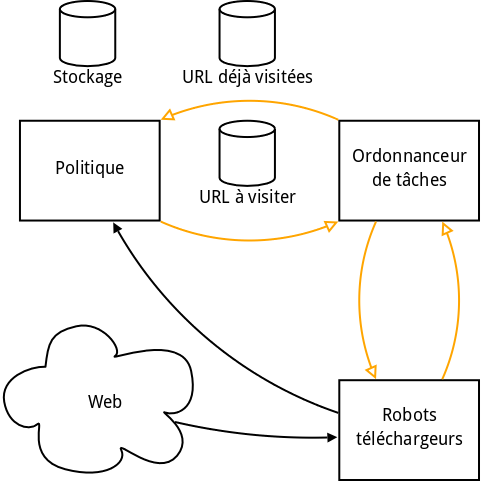
\includegraphics[height=6.5cm]{crawler.png}
}

\frame{
	\frametitle{Crawler - Extraction}

	\begin{block}<+->{Principe du scraping}
	\uncover<+->{\rtgicolor<.>{Analyser une page web pour en extraire une information spécifique}}
	\end{block}

	\begin{block}<+->{\rtgicolor<.>{Problèmes}}
	\begin{itemize}[<+-| rtgicolor@+>]
    \item Validité du code \texttt{HTML}
    \item Encodage
	\item \texttt{DOM} ou Regexp ou les deux
	\item Template et dynamisme des pages scrapées 
    \item Flash et Javascript
	\end{itemize}
	\end{block}
}

\frame{
	\frametitle{Crawler - Difficultés}

%	\begin{block}<+->{\rtgicolor<.>{Des problèmes}}
	\begin{itemize}[<+-| rtgicolor@+>]
	\item Adressage
		\begin{itemize}[<+-| rtgicolor@+>]
       	\item Site ou page ? 
		\item Normalisation d'\texttt{URL} (doublons, IDN, \emph{hash fragment})
%        \item Plusieurs permaliens pour un seul contenu (GYM aide un peu)
		\end{itemize}
	\item Politesse
		\begin{itemize}[<+-| rtgicolor@+>]
		\item DoS (\emph{Denial of Service}) : DNS, Serveurs HTTP
		\item Blacklistage officiel (\texttt{robots.txt}, \texttt{sitemap.xml}, etc.)
		\item Blacklistage officieux (\emph{cloaking}, pièges à robot)
		\end{itemize}
	\item Autres...
		\begin{itemize}[<+-| rtgicolor@+>]
        \item \emph{Deep web}
        \item Web privé et contextualisé
		\end{itemize}
	\end{itemize}
%    \end{block}
}

\frame{
	\frametitle{Crawler}
		
	\begin{block}<+->{\rtgicolor<.>{Astuces}}
	\begin{itemize}[<+-| rtgicolor@+>]
    \item Heuristiques, tolérance
	\item Utiliser les \texttt{headers HTTP}
    \item User-agent
    \item \texttt{random} et \texttt{sleep}
%    \item Multi-agent plutôt que multi-thread
	\end{itemize}
    \end{block}

	\begin{block}<+->{\rtgicolor<.>{Principes du \emph{Focused crawler}}}
	\begin{itemize}[<+-| rtgicolor@+>]
	\item Ne télécharger que les pages pertinentes
	\end{itemize}
	\begin{itemize}[<+-| rtgicolor@+>]
	\item Indicateurs topologiques
	\item Indicateurs sémantiques
	\end{itemize}
    \end{block}
}


\section{Approche moderne}

\frame{
    \frametitle{Le web évolue}

	\begin{block}<+->{\rtgicolor<.>{}}
	\begin{itemize}[<+-| rtgicolor@+>]
    \item Le web statique devient marginal
    \item Web dynamique : du flux de syndication à publish/subscribe
	\item Web applicatif (réseaux sociaux, sites de contenus, micropublications, etc.)
	\end{itemize}
	\end{block}
}

\frame{
	\frametitle{Aggrégation}

	\begin{block}<+->{Principe}
	\uncover<+->{\rtgicolor<.>{Syndication ou comment \emph{renverser} l'accès aux données}}
	\end{block}

    \begin{block}<+->{\rtgicolor<.>{Avantages}}
    \begin{itemize}[<+-| rtgicolor@+>]
    \item L'information est structurée
    \item Ne capter que les nouveaux contenus
    \end{itemize}
	\end{block}

	\begin{block}<+->{\rtgicolor<.>{Problèmes}}
	\begin{itemize}[<+-| rtgicolor@+>]
	\item Atom, \texttt{RSS}, encore mille versions
	\item Flux complet / partiel / vide avec ou sans date, permaliens, \texttt{HTML} 
    \item Pull
	\end{itemize}
	\end{block}

	\begin{block}<+->{\rtgicolor<.>{Solution ?}}
	\uncover<+->{\rtgicolor<.>{Le paradigme publish/subscribe et l'homogénéisation}}
	\end{block}

}


\frame{
	\frametitle{Les API}

	\begin{block}<+->{Principe}
	\uncover<+->{\rtgicolor<.>{Utiliser les API de certains sites pour collecter la donnée}}
	\end{block}

    \begin{block}<+->{\rtgicolor<.>{Avantages}}
    \begin{itemize}[<+-| rtgicolor@+>]
    \item L'information est \emph{vraiment} structurée
    \item Mode de captation recommandé
    \end{itemize}
	\end{block}

	\begin{block}<+->{\rtgicolor<.>{Problèmes}}
	\begin{itemize}[<+-| rtgicolor@+>]
	\item Limitations
	\item Autant de clients que d'API 
	\end{itemize}
	\end{block}

	\begin{block}<+->{\rtgicolor<.>{Solution ?}}
	\uncover<+->{\rtgicolor<.>{SPORE : Specifications for a POrtable Rest Environment}}
	\end{block}

}

\frame{
    \screenshot{github.png}
}

\frame{
	\frametitle{Conclusion}


	\begin{itemize}[<+-| rtgicolor@+>]
	\item Savoir ce que l'on veut récupérer
	\item Choisir la façon la plus structurée
    \item Multiplier les approches
 	\end{itemize}
}

\frame{
	\frametitle{Wikipédia est ton ami :)}

	\begin{itemize}
	\item \url{http://en.wikipedia.org/wiki/HTML}
	\item \url{http://en.wikipedia.org/wiki/Web_crawler}
	\item \url{http://en.wikipedia.org/wiki/Focused_crawler}
	\item \url{http://en.wikipedia.org/wiki/Web_scraping}
    \item \url{http://en.wikipedia.org/wiki/URL_normalization}
	\item \url{http://en.wikipedia.org/wiki/Cloaking}
    \item \url{http://en.wikipedia.org/wiki/User_agent}
    \item \url{http://en.wikipedia.org/wiki/Spider_trap}
	\item \url{http://en.wikipedia.org/wiki/Denial-of-service_attack}
    \item \url{http://en.wikipedia.org/wiki/Atom_(standard)}
    \item \url{http://en.wikipedia.org/wiki/PubSubHubbub}
    \item etc.
	\end{itemize}
}

\frame{
	\frametitle{Merci !}	

    \begin{itemize}
    \item \url{http://labs.linkfluence.net/}
    \item \url{http://github.com/cmaussan/captation-ic05-p11-tex}
    \item \url{http://github.com/cmaussan/Micrawler}
    \end{itemize}

    \pause
}

\end{document}
